% A3-E ideal evaluation
% Awareness: performance and D&A overhead
% Acquisition:performance comparison (ours vs ENORM) 
% Allocation: performance comparison (AWS cold start vs pro-active)
% Execution: service latency and availability comparison 
% ALL: 

\section{Experimental Evaluation}\label{sec:evaluation}

We performed different experiments using four domains that materialize the continuum. 
%The first experiment evaluates $\mu$-service latency against different workloads. 
The first experiment studies how latency changes and how the remote domains scale with a varying workload. 
In this case the mobile domain is obviously omitted. The second one evaluates the domains from a client's perspective, both in terms of latency and battery consumption. The third one evaluates the A3-E with domains that change their availability according to a probability distribution. Finally, the last one evaluates the A3-E's Acquisition and Allocation performance. When possible, we compared A3-E against Enorm, a framework for edge resource management.
%Our goal was to demonstrate that the A3-E model is successful in selecting domains at run time and in improving the overall application availability. 

\subsection{Experiments Setup}

%\subsubsection{Domains}

As shown in Table~\ref{tab:domain-exp-config}, our model was evaluated with four types of domains: mobile, local-edge, and cloud. The client application emulates an Augment Reality one by invoking
%is an Image Recognition one, in which users can capture an image and invoke 
$\mu$-services~\footnote{Implementation available in \url{https://github.com/deib-polimi/A3-E-image-recognition}} responsible for \textit{feature extraction} and \textit{object detection}, which are placed along the continuum. AR is a typical use case for the continuum due to the low latency and high computational power requirements~\cite{beck2014mobile}.

The mobile domain was deployed to an Android smartphone hosting the A3-E middleware. 
%~\footnote{Implementation available in \url{https://github.com/deib-polimi/A3-E-DSM-mobile}}
A domain manager prototype
%~\footnote{Implementation available in \url{https://github.com/deib-polimi/A3-E-DSM-Local-edge}} 
was deployed on two Local-edge domains. For handling Allocation and Execution, we adopted Apache OpenWhisk, a state-of-the-art open-source FaaS platform. Throughout experiments, edge domains shared a LAN with the origin of requests (i.e., the client applications/devices).
%TODO [Danilo] this is by definition and couldn't be otherwise
%This was done to emulate a few-hops scenario in which devices are directly connected to their nearest edge domains. 
\texttt{Local-edge-1} represented a situation in which latency is close to zero, but the computational resources are more constrained and scaling-up is not possible due to the inherent physical restrictions of the underlying infrastructure (e.g., a lightweight server covering an office); in turn, \texttt{Local-edge-2} has more computational resources and yet low latency can be achieved due to physical proximity (e.g., a robust edge server covering a building floor).

Representing cloud domains, we used AWS Lambda~\cite{AWSLambda}, the most mature FaaS solution on the market. To be consistent with our formulation of the compute continuum, functions and associated dependencies (storage, feature extraction and matching) were hosted within the same AWS region. 

Finally, we also deployed the functionality onto a traditional setup using cloud's IaaS. The main goal of this setup was not to compare traditional cloud services against a FaaS solution, but to demonstrate that the proposed continuum could outperform the cloud under the tested circumstances and requirements.

\begin{table}[htb]
	\caption{Domains Setup in the Continuum for the Experimental Evaluation}
	\label{tab:domain-exp-config}
	\footnotesize
	\begin{tabular*}{1\textwidth}{@{\extracolsep{\fill}}>{\raggedright}p{1.7cm}>{\raggedright}p{6cm}>{\raggedright}p{5cm}}
		\toprule 
		Domain & Machine Resources & Execution Environment\tabularnewline
		\midrule
		\midrule 
		Mobile & Samsung Galaxy S6 SM-G90, 3Gb RAM, 8x Cortex CPU 2Ghz & Android 5.0.2 + Java Functions + OpenCV
		\tabularnewline
		\midrule 
		Local-edge-1  & ubuntu/trusty64-2, 4x vCPUs, 4Gb RAM & OpenWhisk, 256 Mb/Action, Python 2.7 + OpenCV \tabularnewline
		\midrule 
		Local-edge-2  & ubuntu/trusty64-2, 8x vCPUs, 16Gb RAM & OpenWhisk, 256 Mb/Action, Python 2.7 + OpenCV \tabularnewline
		\midrule 
		Cloud-FaaS & N/A & AWS Lambda, 256 Mb/Function, Python 2.7 + OpenCV \tabularnewline
		\midrule 
		Cloud-IaaS & Auto Scaling Group with t2.micro instances + Amazon Linux AMI 2017  & NodeJs 6.11 server + Python 2.7 + OpenCv
		\tabularnewline
		\bottomrule
	\end{tabular*}
\end{table}



\subsection{Latency and Scalability} 


%\begin{figure}[htb]
%	\centering
%	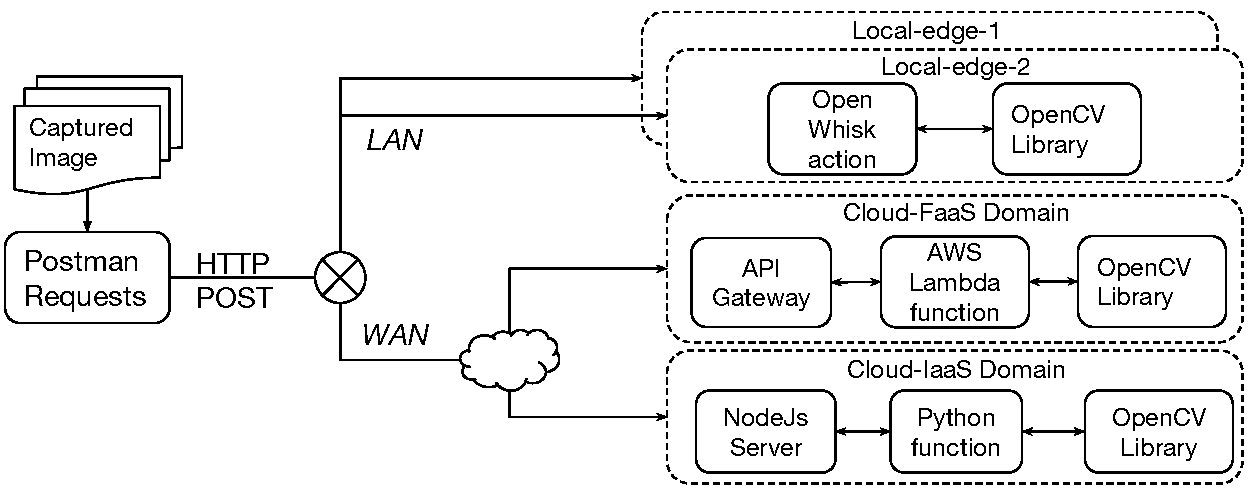
\includegraphics[width=0.95\textwidth]{figs/experimental-setup.pdf}
%	\caption{Setup for Domain Latency Experiments}
%	\label{fig:exp-setup1}
%\end{figure}

The first experiment assessed how the latency changes and the domains scale with a varying workload, providing a baseline to compare different domains. We simulated an increasing number of clients, each one making $100$ requests for the AR $\mu$-service at a rate of two per second. This setup was achieved taking into account the default maximum for concurrent executions in AWS Lambda~\cite{AWSLambda}
%~\footnote{\url{http://docs.aws.amazon.com/lambda/latest/dg/concurrent-executions.html}} 
and Openwhisk~\cite{OpenWhisk}.
%~\footnote{\url{https://github.com/apache/incubator-openwhisk/blob/master/docs/reference.md}}, as well as the limited resources of edge domains. 

This experiment excluded the mobile domain and focused on the remote ones, i.e., edge and cloud. Capturing and uploading an image was emulated using Postman\footnote{\url{https://www.getpostman.com/}}, an open source application designed to perform load testing over the functional behavior of Web APIs. The payload for this experiment was a sample image of approximately 65 KB, which is a reasonable size for this use case considering the requirements regarding low-latency and computation time~\cite{rodriguez16mobile}. The actual execution time was profiled for each domain and then kept constant for the experiment, while latency results are averaged through $5$ executions.

%Once the image was sent through HTTP/POST, the actual execution depended on the domain being used. triggering Openwhisk actions for both edge domains, AWS Lambda functions for Cloud-FaaS domain, and a Nodejs server that calls a Python function for Cloud-IaaS domain.

%was performed without using the A3-E middleware nor the device (mobile domain), since it aims to evaluate the plain latency for remote domains when processing simultaneous requests. This scenario would not occur in a mobile domain, which only process local requests. The possibility of offloading computation from one mobile device to another is left as a future work.

%In our edge domains for the experiment, uploading an image to CouchDB (Step 3.a) triggers the action that performs the feature extraction and matching (Step 4.a)  with the points-of-interest, supported by the OpenCV\footnote{\url{http://opencv.org}} visual recognition library (Step 5.a). 




%\subsubsection{Baseline Latency}

Fig.~\ref{fig:latency-domains} shows the average latency for each scale-up step. Note that the computation time (light gray) is different from the overhead (dark gray). The latter includes network communication (routing and forwarding) and queuing time (when no resources are available to process the request immediately). 

\begin{figure}
	
	\centering
	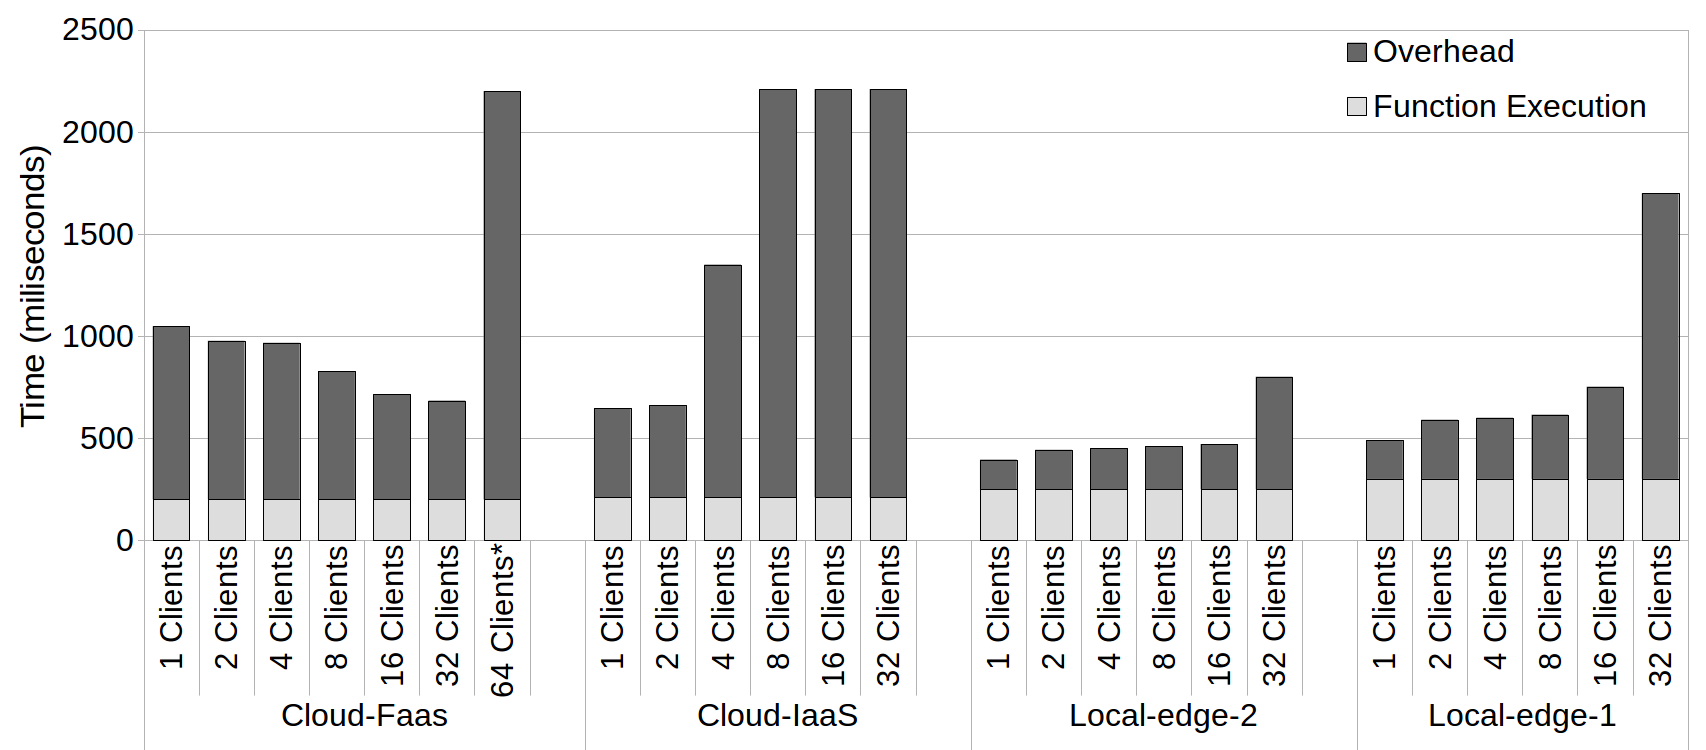
\includegraphics[width=.9\textwidth]{figs/latency-domain-new}
	\scriptsize{(*)max-concurrent-executions = 64}
	\vspace{-.3cm}
	\caption{Latency and scalability for each domain and different number of clients.}
	\label{fig:latency-domains}
\end{figure}

Regarding the \textit{Cloud-FaaS} domain, the latency reduction is up to $90$\% for \texttt{Local-edge-1} and up to $82$\% for \texttt{Local-edge-2}. Interestingly, for Cloud-FaaS, latency decreases when the number of simultaneous clients increases.
This is due to the fact that extra infrastructure is provisioned under-the-hood by AWS Lambda to compensate for initialization overhead of cold requests. Even though future service requests against warm infrastructure do not always reuse extraneous infrastructure created in response to cold initialization stress, higher reuse rates correspond with higher stress levels of requests~\cite{Lloyd18serverless}. For few service invocations, load distribution by AWS is uneven across hosts. This uneven use of infrastructure may lead to early deprecation (incurring in cold starts) if client workloads do not utilize all nodes. 
Despite its virtually unlimited resources, Cloud-FaaS has tunable limits for maximum concurrent executions (default is 1000), e.g., due to budget constraints~\cite{Villamizar2017lambda}. This is reflected in the substantial increase in latency noticed in the Cloud-FaaS experiment (Fig.~\ref{fig:latency-domains}, Cloud-FaaS, 64 Clients bar), performed with 64 clients and similar concurrent execution limit.
%We run an additional scenario for Cloud-FaaS to reflect the situation in which such a limit is reached, with 64 clients and 64 maximum concurrent executions. 
%, perceived latency increases substantially as the requests are throttled by the infrastructure.

Regarding the \textit{Cloud-IaaS} domain, reductions when using \textit{Cloud-FaaS} are up to $77$\% and $58$\%, respectively. Interestingly, \textit{Cloud-IaaS} outperformed  \textit{Cloud-FaaS} ($46$\% less overhead) for light workloads (up to $16$ simultaneous clients). This can be due to the additional steps performed by the API Gateway in order to forward RESTful calls to AWS lambda functions in \textit{Cloud-FaaS}\footnote{http://docs.aws.amazon.com/lambda/latest/dg/with-on-demand-https.html}. Nevertheless, this advantage is mitigated by the fact that \textit{Cloud-FaaS} can better react to workload bursts, thanks to its faster horizontal scaling~\cite{Villamizar2017lambda,Hendrickson:2016}. 
%[Danilo] the cited works should be enougth for explaining why
%Since in \textit{Cloud-IaaS} a scaling-up action (that can demand several seconds~\cite{Quatrocchi2016discrete}) triggers when more than one VM instance is needed to handle the workload, requests timeout in the meantime. 
 
For light to medium workloads (up to $16$ simultaneous clients), the overhead added by the \textit{Local-edge} domains is less than both cloud alternatives. Under heavier workloads (from $32$ simultaneous clients onwards) these domains present restricted availability and degraded performance -- as can be seen for \texttt{Local-edge-1} (the most resource-constrained). One may argue that a \texttt{Local-edge} domain is intended to cope with light workloads -- e.g., a single office or floor in a building. For edge domains that may cope with hundreds of simultaneous clients, e.g., a mobile-edge domain, the compute, storage and memory capabilities are expected to be orders of magnitude higher.
 
Finally, we compared our \texttt{Local-edge-2} deployment against Enorm~\cite{wang2017enorm}, a framework for edge resource management that assumes a similar, resource constrained configuration for the edge nodes. %(details are discussed in Section~\ref{sec:related}). 
Fig.~\ref{fig:a3e-enorm-latency} shows the latency reduction when using an edge alternative instead of a cloud one. A3-E performs better for up to 32 simultaneous requests (from 35\% to 55\% latency reduction w.r.t. the cloud), whilst both approaches tend to perform worst than the cloud solution with heavier workloads (from 64 simultaneous requests on).  



%\subsection{Battery} The second set of experiments targeted the measurement of battery consumption of a mobile device in two scenarios: 1) in which feature extraction and matching were performed locally, and 2) these tasks were offloaded to edge servers.

\subsection{Battery Consumption and Execution Time} 
\label{sub:exp-a3e-continuum}

The main goal of this experiment was to evaluate the compute continuum 
from the client's viewpoint in terms of battery consumption and execution time. A mobile device was set up with our implementation of the A3-E middleware, which was in charge of selecting the best domain from Table~\ref{tab:domain-exp-config} for serving the sample application $\mu$-service based on the perceived QoS.
%[Danilo] The experiment set-up already defined the application (saving space here)
%Once again our sample application was the image recognition one with feature extraction and matching provided along three domains in the continuum: \textit{mobile}, \textit{Local-edge} and \textit{Cloud-FaaS} (see Table~\ref{tab:domain-exp-config}). 

This experiment featured four different scenarios: the first three consider one domain each, and the last one (\textit{all-domains}) combines the previous ones to form the continuum\footnote{Details on the availability of each domain in the \textit{all-domains} scenario are discussed in Section~\ref{sub:domain-selection}.}. The experiment consisted in cascading $2000$ sequential requests for \textit{feature extraction} and \textit{matching} of a sample image (with a size of 65 KB). We measured the total execution time, battery consumption in the mobile device, and average time per call. Fig.~\ref{fig:exp-a3e} shows the experimental results, averaged among $5$ executions for each scenario.

\begin{comment}
internetOnToOffProbability = 0.22%
internetOffToOnProbability = 1.66%

edgeOnToOffProbability = 3.33%;
edgeOffToOnProbability = 6.66%;

e = 1/p; //average number of trials it takes for the event with probability p to happen
~t = e * u;  //average time it takes for the event with probability p to happen given a trial interval u
~t = u/p; //the same, but using the trial interval and the probability p 

###

trial interval u = 2 seconds

average time for disconnecting: 15 x 60 seconds
prob. of disconnecting: 0.2222222%   

average time for reconnecting: 2 x 60 seconds
prob. of reconnecting: 1.666666%

average time for edge unavailability: 10 x 60 seconds 
prob. of edge unavailability: 0.333333%

average time for edge becoming available: 5 x 60 seconds 
prob. of edge becoming available: 0.666666%

\end{comment}

%(all-domains).



\begin{figure}[htb]
	\centering
	\captionsetup[subfigure]{width=0.32\textwidth}	
	\subfloat[Total execution time (sec)\label{fig:total-exec-a3e}] {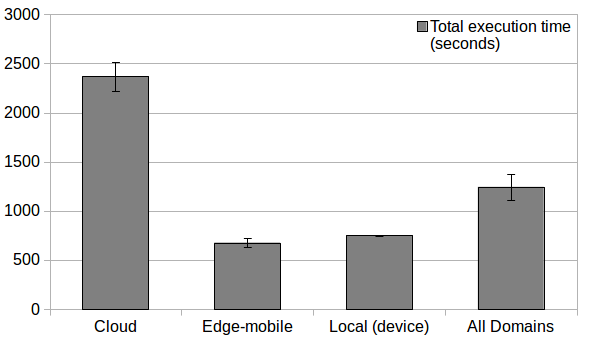
\includegraphics[width=0.32\textwidth]{figs/total-exec-time-A3E}}	\captionsetup[subfigure]{width=0.32\textwidth}
	\subfloat[Battery consumption (\%)\label{fig:battery-a3e}] {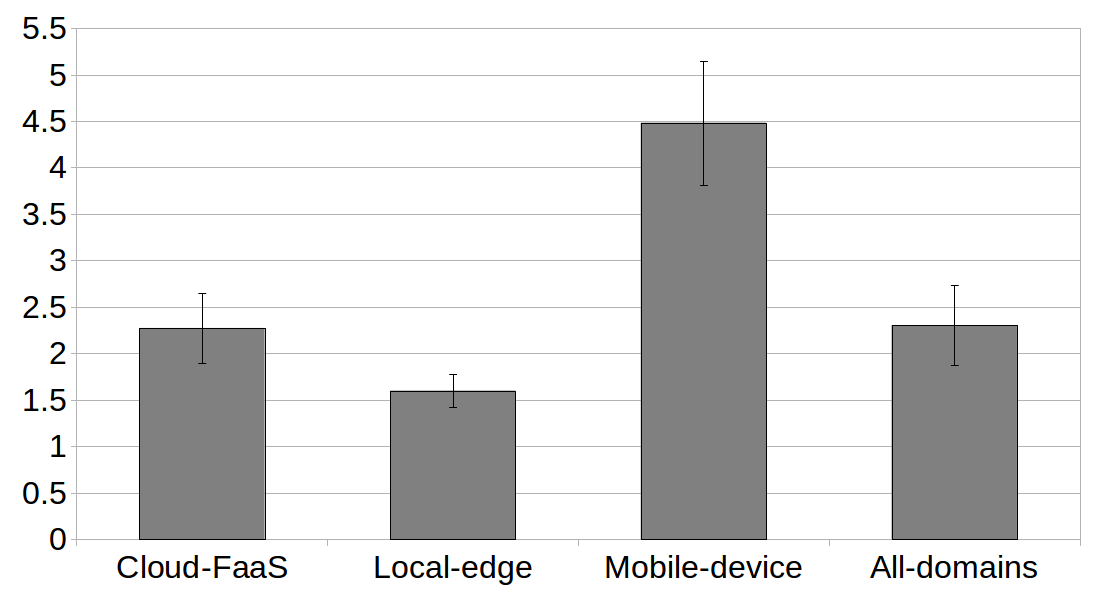
\includegraphics[width=0.32\textwidth]{figs/battery-consumption-A3E}}
	\captionsetup[subfigure]{width=0.32\textwidth}	
	\subfloat[Execution time per call (ms)\label{fig:time-per-call-a3e}] {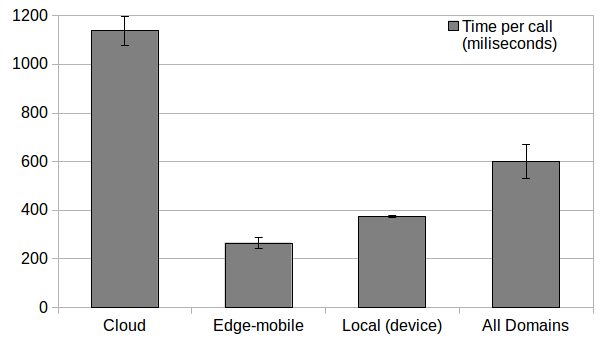
\includegraphics[width=0.32\textwidth]{figs/time-per-call-A3E}}
	%\captionsetup[subfigure]{width=0.45\textwidth}
	%\subfloat[Number of Calls per domain in all-domains scenario\label{fig:calls-per-domain-a3e}] {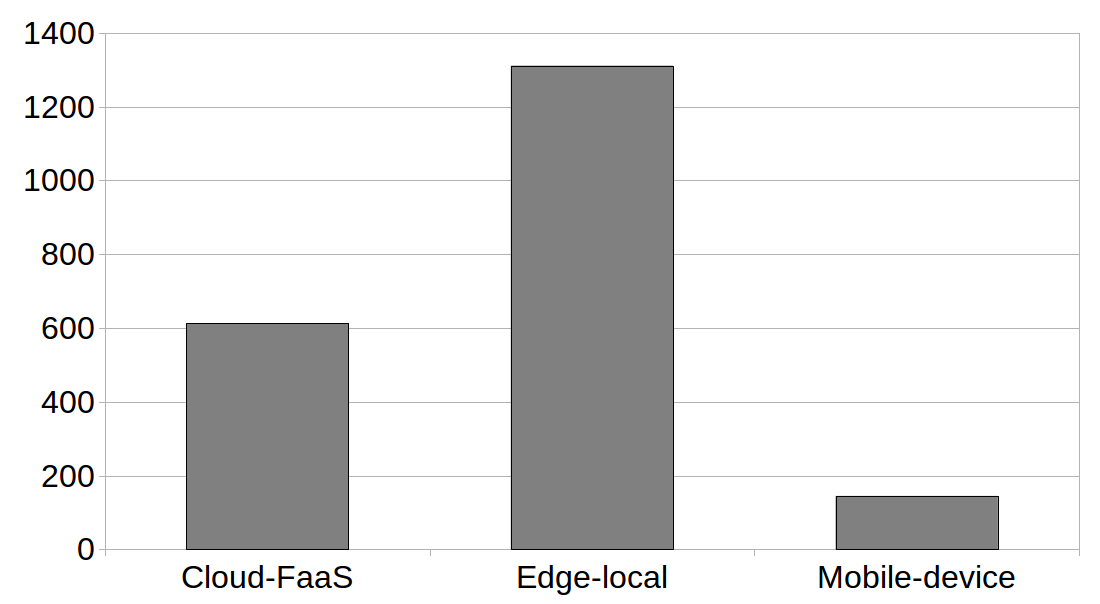
\includegraphics[width=0.45\textwidth]{figs/calls-per-domain-A3E}}
	\setlength{\belowcaptionskip}{-10pt}	
	\caption{A3-E experimental evaluation results} \label{fig:exp-a3e}
\end{figure}

%\begin{figure}[htb]
	%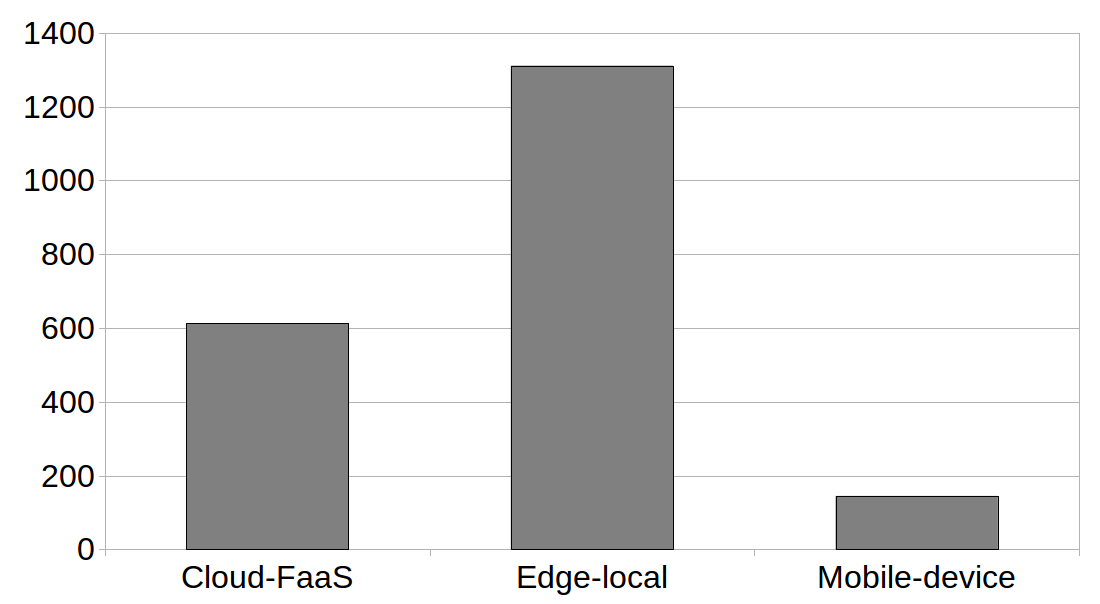
\includegraphics[width=0.45\textwidth]{figs/calls-per-domain-A3E}
	%\caption{Number of Calls per domain in all-domains scenario}
	%\label{fig:calls-per-domain-a3e}
%\end{figure}

For the total execution time (Fig.~\ref{fig:total-exec-a3e}), considering the \texttt{Cloud-FaaS} domain as a baseline, \texttt{Local-edge} reduced it up to a $72$\%, while \texttt{mobile} and \texttt{all-domains} up to a $69$\% and $49$\%, respectively. In turn, the baseline for battery consumption (Fig.~\ref{fig:battery-a3e}) was measured with the \texttt{mobile} domain and resulted in a battery drop of $4.5$\% after $750$ seconds (i.e., $12.5$ minutes) of execution. Battery savings with \texttt{Cloud-FaaS}, \texttt{Local-edge} and \texttt{all-domains} were $49$\%, $35$\%, and $49$\%, respectively. The time per call (Fig.~\ref{fig:time-per-call-a3e}), with \texttt{Cloud-FaaS} as our baseline ($1137$ milliseconds per call), was improved by $76$\%, $68$\% and $47$\% for \texttt{Local-edge}, \texttt{Mobile} and \texttt{all-domains}, respectively. 

These experiments tell us that the total execution time, when using only the cloud, was two times higher than when using the continuum (\texttt{all-domains}). Since the requests were performed in cascade and given the higher latency per call in the cloud, the total time increases accordingly. Clearly, using A3-E to switch to edge domains when possible substantially reduces the latency and improves the perceived QoS.

Battery consumption was substantially lower when offloading computation, rather than performing it on the device. The \texttt{mobile}-device scenario lasted half the time, but used twice as much battery (a prohibitive $20$\% of battery drain per hour) than the \texttt{all-domains} one, given that it was performing CPU intensive operations. This recalls the importance of computation offloading to preserve mobile device's resources.

\subsection{Domain Selection and Availability}
\label{sub:domain-selection}

We evaluated the capability of A3-E to select the best domain given low latency and high computational power requirements. In this experiment, we used all three domains together to form the continuum and simulated their availabilities after a probability distribution. 

The mobile middleware was configured to ping for domain availability, as well as perceived QoS, every two seconds ($u = 2$). We consider that the cloud domain could be unavailable mainly due to absence of mobile network coverage, since downtimes of cloud services are minimal~\cite{garcia2017bandwidth}. To simulate this, the average network unavailability was set to once every $15$ minutes. Then, the average time for it to become available was $2$ minutes, which gives us an availability of $88\%$.

%\footnote{https://math.stackexchange.com/questions/165993/average-number-of-times-it-takes-for-something-to-happen-given-a-chance}
The rationale for the edge domain is analogous, yet with a higher probability of being unavailable (e.g., due to the lack of resources or connectivity). In this case, the edge is unavailable once every $10$ minutes, and it would take an average of $5$ minutes for it to become available, which gives a $66\%$ of availability. If we consider that edge nodes are only reachable within network coverage, the resulting availability is calculated by their product, or $0.88*0.66=58\%$. The mobile device is considered as always available, and selected when all other domains were unavailable, or the sensed latencies were too high for the application's QoS requirements. 

%To simulate the cases in which the mobile device was momentarily outside of the mobile network's coverage, the average unavailability of the cloud domain~\cite{garcia2017bandwidth} was set to once every $15$ minutes. A3-E was configured to ping for domain availability, as well as perceived QoS, every two seconds ($u = 2$). Using a geometric distribution, the probability of the cloud being unavailable during a ping (\textit{internetOnToOff}) was $0.022$. Every time the cloud was unavailable, the average time for it to become available again was $2$ minutes, i.e., the probability  \textit{internetOffToOn} was $0.166$. Overall, this gives us a probability \textit{internetAvailability} $=15/(15+2)=0.88$.

%\footnote{https://math.stackexchange.com/questions/165993/average-number-of-times-it-takes-for-something-to-happen-given-a-chance}

%The rationale for the edge domain is analogous, yet with a higher probability of it being unavailable --- e.g., due to the lack of physical proximity with the edge servers. In this case, the edge is unavailable once every $10$ minutes, i.e., the probability was \textit{edgeOnToOff}  $ = 0.33$. Once unavailable, we considered that it would take an average of $5$ minutes for it to become available again, i.e. the probability \textit{edgeOffToOn} was $0.066$. Therefore, the probability \textit{edgeAvailability} $=10/(10+5)=0.66$. If we consider that edge nodes are only reachable within network coverage, then the probability \textit{edgeAvailabilityWithAvailable}$=0.88*0.66=0.58$.

In order to set an \emph{optimal} baseline for this experiment, we calculated the theoretical number of calls to be served per domain, given the probabilities explained above. Upon this, the \emph{optimal} execution time was calculated, assuming no overhead for domain switching and always using the best domain available.

Fig.~\ref{fig:all-domains} shows detailed results for the \texttt{all-domains} scenario w.r.t. availability and consistency. The experiment shown (see Fig.~\ref{fig:availability-all-domains}) an average of $93\%$ perceived availability without considering the \texttt{mobile} domain ($5\%$ and $35\%$ improvement regarding cloud and edge respectively), and $100\%$ availability when considering also the \texttt{mobile} domain (which is always available). 

Fig.~\ref{fig:calls-per-domain-a3e} shows the distribution of calls per domain in the continuum: $63\%$ by \texttt{Local-edge}, followed by \texttt{Cloud-FaaS} ($30\%$) and \texttt{mobile} ($7\%$) -- with an optimal of $66$, $22$ and $12\%$ respectively. In terms of consistency, given that all requests were served, on average $70\%$ of the requests perceived low latency, whilst the $30\%$ that relied on the cloud perceived a degradation in QoS but still were processed successfully. Finally, Fig.~\ref{fig:total-exec-time-optimal} shows an increase of $33\%$ in the total execution time using A3-E w.r.t. the optimal, where the former includes the overhead of domain selection and switching.
 
\begin{figure}[htb]
\centering
	\captionsetup[subfigure]{width=0.32\textwidth}
	\subfloat[Average availability (\%)\label{fig:availability-all-domains}] 
	{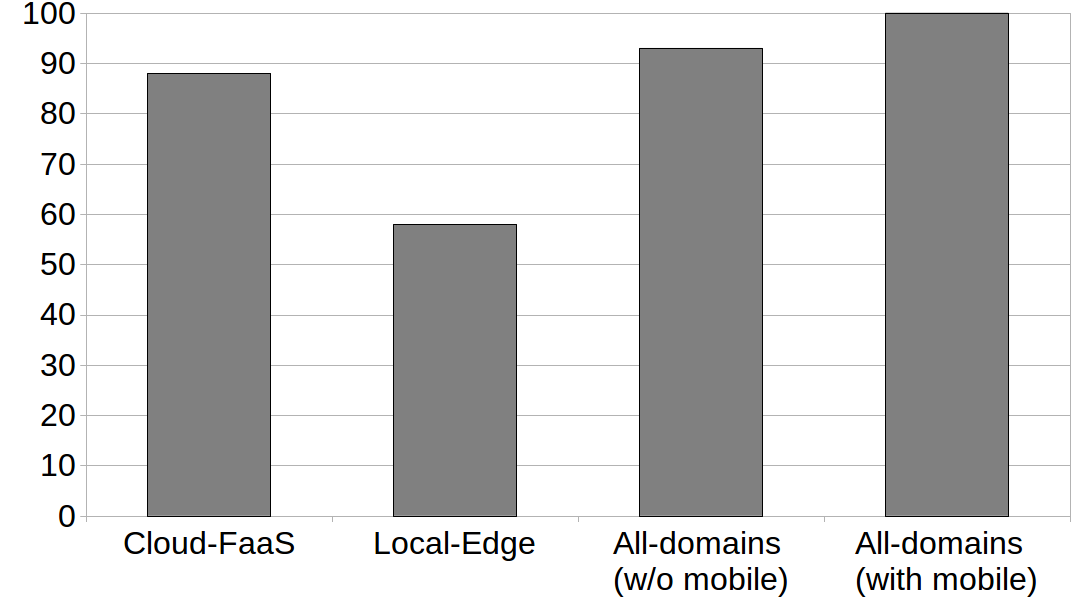
\includegraphics[width=0.32\textwidth]{figs/availability-all-domains}}
	\captionsetup[subfigure]{width=0.32\textwidth}
	\subfloat[Number of requests served\label{fig:calls-per-domain-a3e}] {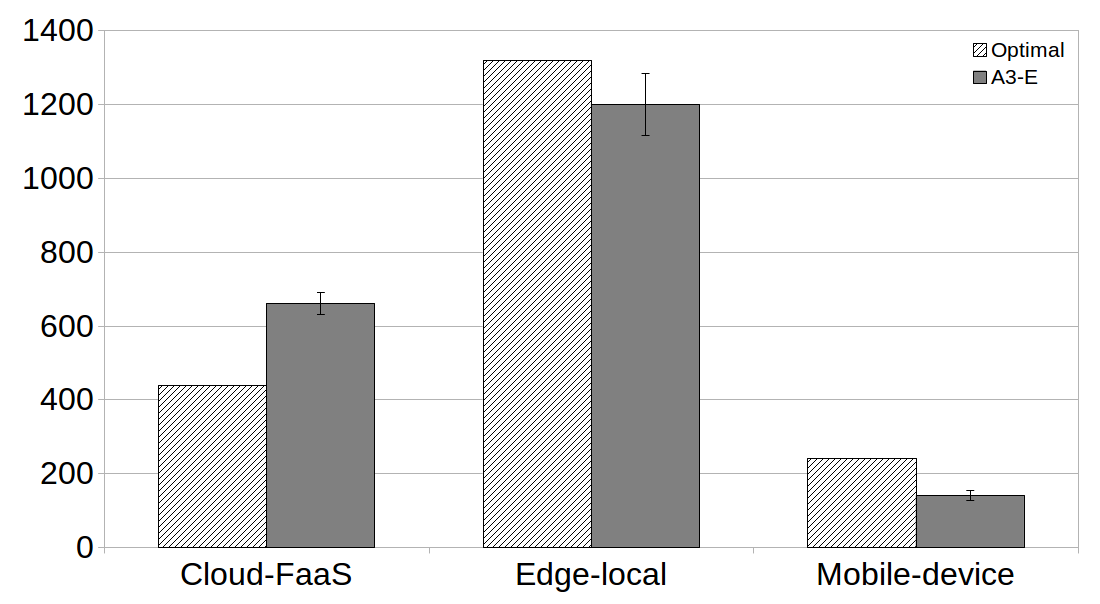
\includegraphics[width=0.32\textwidth]{figs/calls-per-domain-A3E-optimal}}
	\captionsetup[subfigure]{width=0.32\textwidth}
	\subfloat[Total Execution Time (sec)\label{fig:total-exec-time-optimal}] {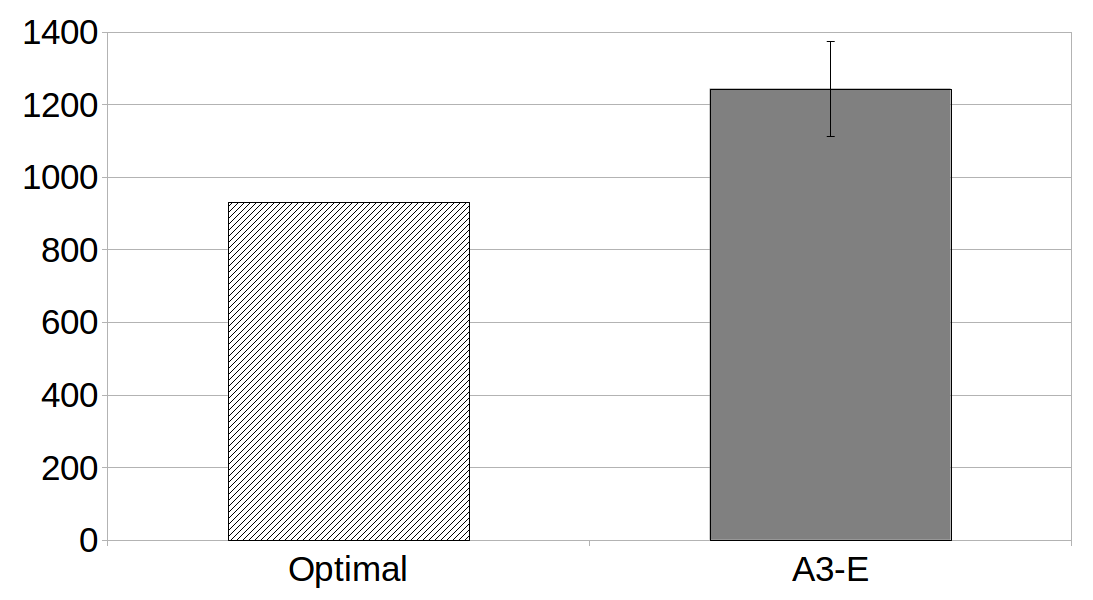
\includegraphics[width=0.32\textwidth]{figs/total-exec-time-optimal}}
	\setlength{\belowcaptionskip}{-10pt}
	\caption{All-domains scenario results} \label{fig:all-domains}
\end{figure}

Conclusively, the experiment shown that A3-E is capable of performing domain selection and computation distribution at runtime. A3-E also improved availability up to 100\% during the experiment, given that the mobile domain is always available, but selected to serve only 7\% of the requests.
The \texttt{all-domains} scenario reflects the underlying rationale of the computation continuum: exploit the edge domains as much as possible (by giving them high scores in Formula~\ref{eq:smart}), leading to better balance among computation time, latency and resource consumption. 
%[Danilo] is the sentence below meanigful?
%Switch to the cloud, or to the local device, only when necessary. 
Note that computation in the mobile device was configured with the lowest possible score, thus the cloud was selected as the first alternative to edge domains. This behavior can be tuned by adjusting application requirements and domain parameters as discussed in Section~\ref{sec:implementation}.

%that allows to cope with unavailability and fluctuations in QoS 

%\textcolor{blue}{TODO:(2) Discuss the relevance of the results }

%\paragraph{Threats to validity}

\subsection{Opportunistic Acquisition and Allocation through Awareness}

Finally, the last experiment evaluates the performance of A3's Acquisition and Allocation based on Awareness. Given the resource limitations of edge domains and the potential benefits of exploiting contextual awareness related to edge's locality, we target the evaluation of \textit{Local-edge-2} as a domain. 

The experiment focused on the scenario in which no edge resources are pre-allocated beforehand, i.e., a worse case cold-start scenario (see Section~\ref{sec:A3-E-awareness}). In this context, the experiment was carried out with a prototype implementation of a domain manager responsible for the advertisement, identification, acquisition and allocation of a new $\mu$-service by that domain.

% [Danilo] The steps are described in Sec. 3, we can just emphatise the activities (paragraph above)
%the following steps: (1) Receive a client's request targeting a new $\mu$-service, (2) fetch and download the software assets from a repository, (3) build the $\mu$-service against the specific architecture of the edge node (if needed), (4) install the corresponding functions in the FaaS platform and provide an endpoint for them, and finally (5) execute the requested function and return the result to the client.

The sample $\mu$-service was similar to previous experiments. Comprising the \textit{client identification} signal, the client informs the server regarding the repository to fetch the required assets (~30 Mb including the $\mu$-service function and dependencies).
%, activity that is delayed until after the first function call due to the opportunistic policy. 
Also, note that the experiment measures only domain-side performance, as latency perceived by clients was evaluated in the previous experiments. After a successful Acquisition and Allocation, we uninstalled and deleted all the $\mu$-service assets, so that subsequent iterations also captured a worse case cold-start.

The experiment execution consisted of cascading sequential requests for periods of $5$ minutes, with different utilization levels of the edge node: low (~10\% server load and low network traffic equivalent to 8 clients), medium (~55\% server load and 16 clients) and high (~85\% server load and 32 clients). Again, we were able to compare A3-E against the Enorm framework, given that A3-E's Acquisition and Awareness are analogous to the provisioning phase in Enorm, which consists of deploying application server partitions from the cloud to edge node containers. 

\begin{figure}[htb]
	\centering
	\captionsetup[subfigure]{width=0.49\textwidth}
	\subfloat[Latency Reduction (\%)\label{fig:a3e-enorm-latency}] 
	{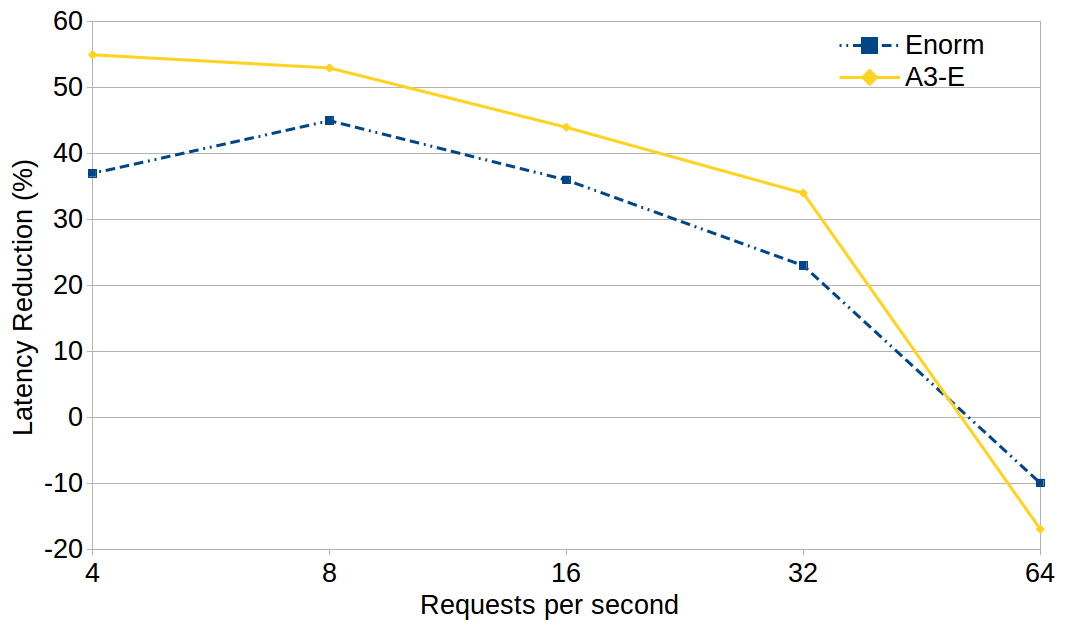
\includegraphics[width=0.49\textwidth]{figs/a3e-enorm-latency}}
	\captionsetup[subfigure]{width=0.49\textwidth}
	\subfloat[Provisioning Overhead (sec)\label{fig:exp-a3e-enorm-deployment}] {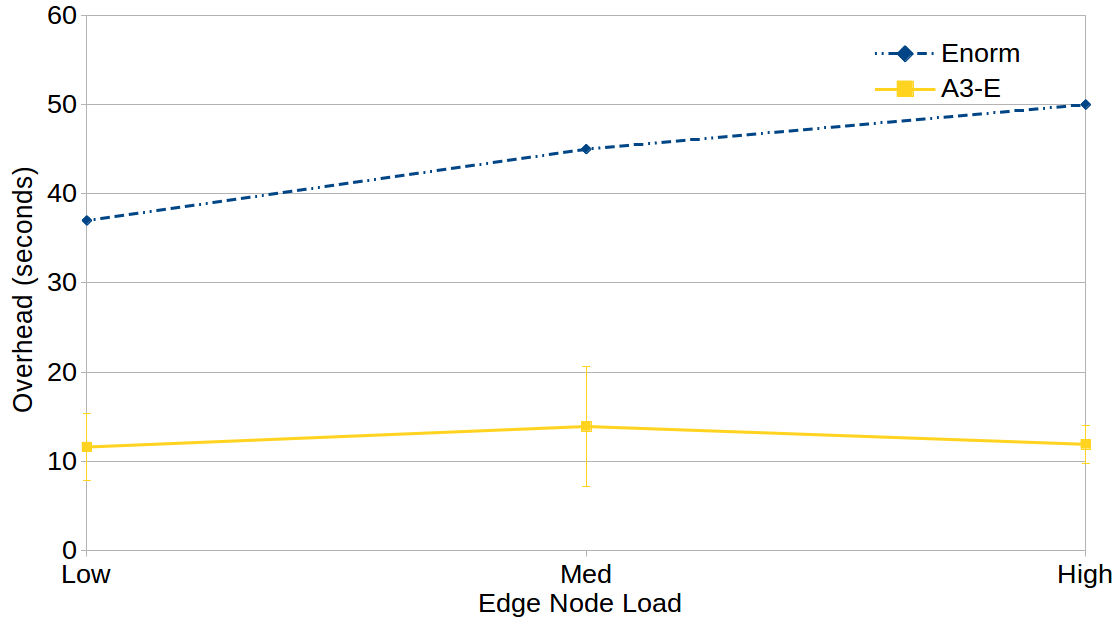
\includegraphics[width=0.49\textwidth]{figs/a3e-enorm-deployment}}
	\setlength{\belowcaptionskip}{-10pt}
	\caption{Comparison of A3E and Enorm when using an edge alternative instead of the cloud.} \label{fig:exp-a3e-enorm}
\end{figure}


\begin{comment}
\begin{figure}	
	\centering
	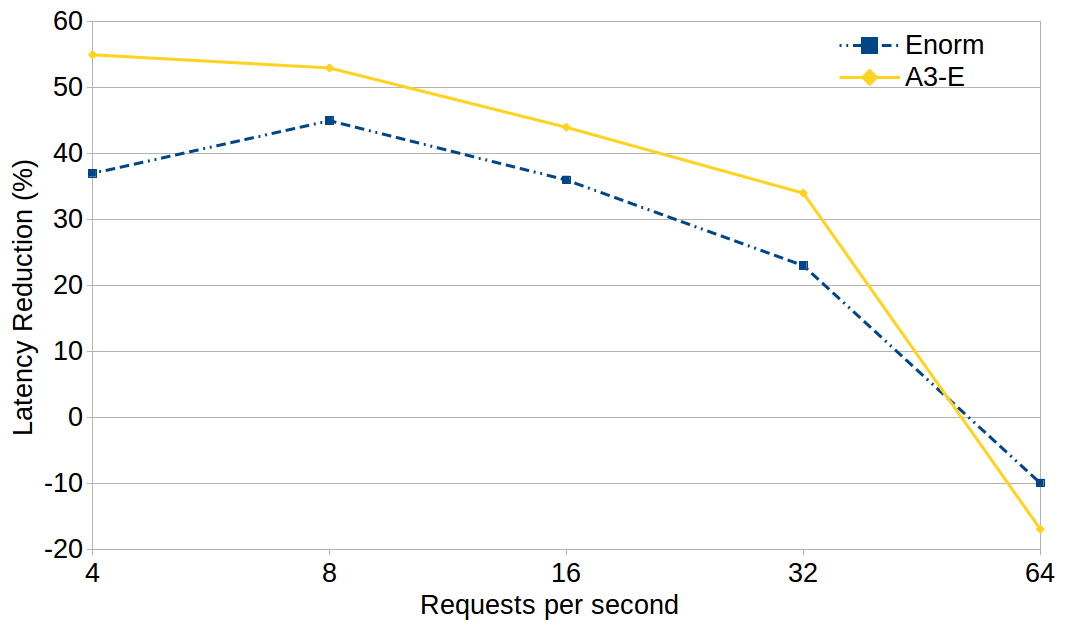
\includegraphics[width=.9\textwidth]{figs/a3e-enorm-latency}
	\vspace{-.3cm}
	\caption{Latency improvements for A3E and Enorm when using an edge alternative instead of the cloud.}
	\label{}
\end{figure}


\begin{figure}	
	\centering
	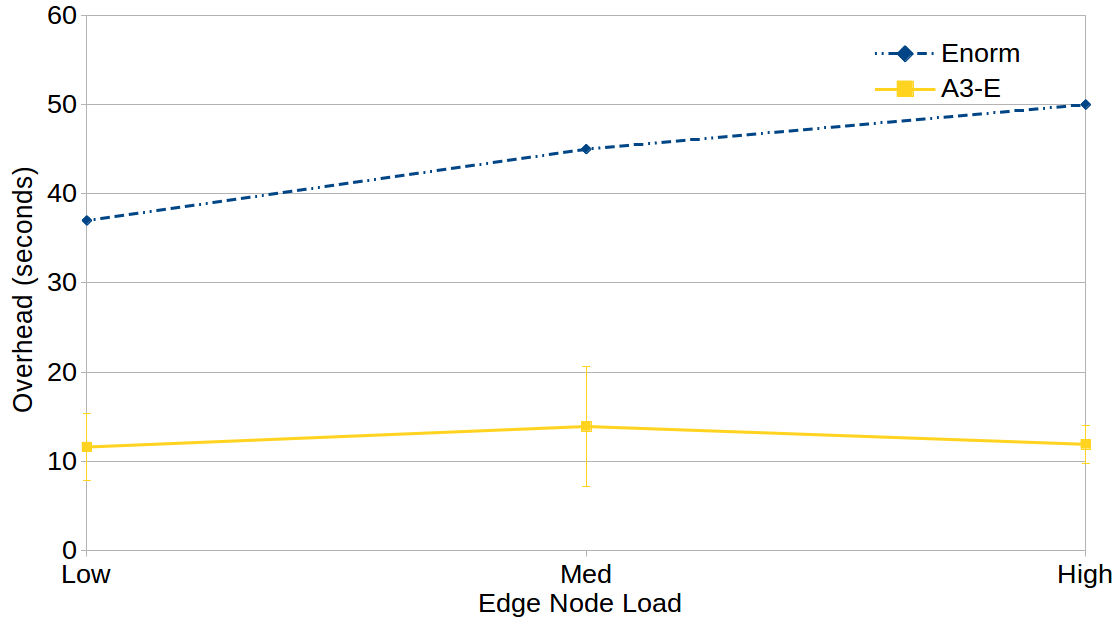
\includegraphics[width=.9\textwidth]{figs/a3e-enorm-deployment}
	\vspace{-.3cm}
	\caption{Overhead for A3E (Acquisition and Allocation phases) and Enorm when provisioning new functionality to an edge node.}
	\label{}
\end{figure}
\end{comment}

Fig.~\ref{fig:exp-a3e-enorm-deployment} shows the experiment results. The average time between detection of a \textit{client identification} event and successful Allocation was 12.5 and 44 seconds for A3-E and Enorm respectively, without considerable variations regarding the current load of the edge node. Such a reduction of provisioning overhead (up to 70\% less) is one of the main advantages of adopting a FaaS model for the continuum. The underlying FaaS solution (OpenWhisk in this experiment) reduces the burden of downloading and installing new functionality: thanks to the highly shared platform, $\mu$-service functions can be created and deleted in a fraction of the time needed to do so with whole containers (as in Enorm and most state-of-the-art solutions). 

%built it in the edge server, and installation of a functionwe used the Image Recognition function from the Augmented Reality application 


Finally, in terms of threats to validity is it worth mentioning that the experiments only targeted one sample application and, in the case of experiments in Section~\ref{sub:exp-a3e-continuum} and~\ref{sub:domain-selection}, only one client device. Further tests are needed, considering multiple clients using several applications composed of $\mu$-services with conflicting requirements, and their corresponding functions deployed along the continuum. Additionally, it is currently not possible to test with real mobile-edge domains, i.e., to provide computational capabilities on base stations. This could be approximated either by simulation or by deploying edge domains following current specifications of \textit{mobile edge computing} in terms of computational power and latency, to better capture the heterogeneity of the continuum. Nonetheless, the fact that specifications and technologies are still under development limits the accuracy in which mobile-edge domains can be evaluated.  %Finally, even though the all-domains scenario provided insights regarding availability and consistency, experiments focusing particularly on consistency, correctness and reliability of the model are outside the scope of the paper and thus left as future work.



